\begin{figure}[H]  
  \begin{center}
    \includegraphics[width=\linewidth]{./images/fffChannelMeasures.pdf}    
  \end{center}
  \caption[Channel dimensions]{Channel dimensions. The width $b(\zL)$ depends on the focus position and is not 
  accessible via geometrical channel data only.}
  \label{fig:fffChannelMeasures} 
\end{figure}AF4 channel have a trapezoidal shape with measures indicated in fig. \ref{fig:fffChannelMeasures}.
For all further considerations, the channel plane is split into three sections (1,2,3) with their correspoding lengths $L_1, L_2, L_3$. To simplify the further calculations, they are subsumed as in the following:
% \begin{itemize}
% \item the widths at the channel intersections
% \item the three lenghts $L_1$, $L_2$ and $L_3$ of the channel sections with their sum
% \end{itemize}
\begin{equation}
  % \dot{L}
  L
  = L_1 + L_2 + L_3 = L_{12} + L_3   
\end{equation}
As the sample is focussed at a certain channel position on the beginning, this has to be considered. The relative focus position \zP is related to the other focus-related magnitudes by
\begin{equation}
  z_0 = \zP L = L - \zL
\end{equation}
The channel height difference \bDelta on the section 2 is
\begin{equation}
  \bDelta = b_0 - \bL \geqq 0
\end{equation}

Volume calculation may be conducted for the trapezoidal by simple decomposition of the channel plane into elementary 
geometrical objects. However, a concise analytical approach is more appropriate as the result can be displayed as a 
function of $\zP$. In addition the corresponding $b(\zP)$ is not known initially. Similar derivations have already been 
conducted with the approximation of dividing the shape into two sections.\scite{Wahlund2013, Magnusson2012, 
Bolinsson2018, Haakansson2012}
The approach may be useful for further hydrodynamic considerations as for example, the elution flow $V_e(x)$ in AF4 is 
a position-dependent size. For the trapezoidal plane shape, the channel is described by the enclosure of three pairs of 
straight line \ref{fig:fffChannelCoordSys}. All expressions here are not optimized for mathematical elegance, but 
rather for being translated into an understandable and well-maintainable calculation routine. This is achieved by 
extensive subsitution of the known variables. Subsuming of these magnitudes helps to simplify the later expressions. 
In addition It allows the transformation and variation if a modification is required, for example if and another shape 
model shall be introduced.
Due to the reason of symmetry, only three borders have to described exactly:

\begin{align}
  \frac{1}{2}b(x) = E(x) \left\{  
  \begin{array}{lcrcl}
    \intGreenBox {\ensuremath{ e_1(x) = m_1 x       = \frac{b_0}{2L_1} \cdot x   }}
    & \forall & 0 \leqq & x &\leqq L_1 \\\addlinespace %\label{eq:chLine1} \\
    \intBlueBox {\ensuremath{ e_2(x) = m_2 x + t_2  = - \frac{\bDelta}{2 L_2} \cdot x  + \frac{1}{2} \left( b_0 +  \frac{L_1}{L_2}\bDelta \right)     }}
    & \forall & L_1 < & x &\leqq L_{12}  \\\addlinespace  % \label{eq:chLine2} \\
    \intPurpleBox {\ensuremath{ e_3(x) = m_3 x + t_3  = - \frac{\bL}{2L_3}  \cdot x + \frac{L \bL}{2 L_3 } }}
    & \forall & L_{12} < & x &\leqq L   \\ %  \label{eq:chLine3}
  \end{array}
  \right.
  \label{eq:chLine}
\end{align}
\begin{figure}  
  \begin{center}
    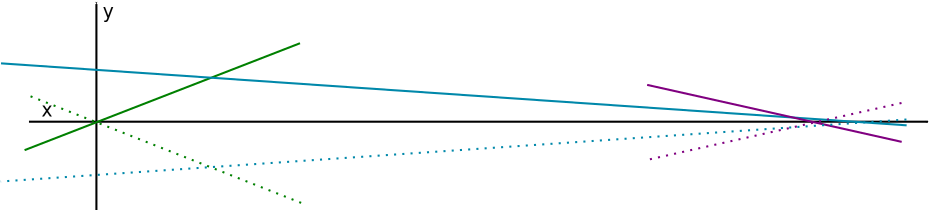
\includegraphics[width=\linewidth]{./images/fffChannelCoordSys.pdf}    
  \end{center}
  \caption[Channel dimensions as a set of straight lines]{Channel dimensions as a set of 3 pairs of straight lines.}
  \label{fig:fffChannelCoordSys} 
\end{figure}
As all dimensions here are known, the slopes and offsets of the lines can be calculated directly and don't have to be resubsituted after the following substitutions.
The calcuation of geometrical volume of the trapezoidal channel has to be adapted according to whether the focus 
position $z_0$ is located left or right to the position of maximal channel extent ( i.e. if $z_0 < L_1$ or $z_0 \geqq 
L_1$). In the algorithm later, rather the plane is used explicitly, which is obtained easily \clearpage
\subsubsection*{\Vgeo: Distal focussing with $\bm{z_0 \geqq L_1}$}
\begin{figure}[h]
  \begin{center}
    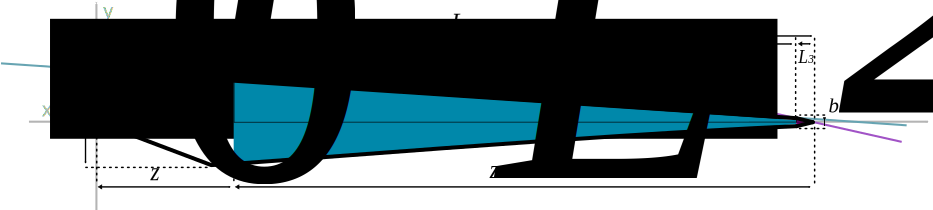
\includegraphics[width=\linewidth]{./images/fffVolume1.pdf}
    \vspace*{-3ex}    
  \end{center}
  \caption[Passed area section - distal focussing]{Area section passed by the sample during the measurement marked with 
  the color of the corresponding line in the case of distal focussing}
  \label{fig:fffVolume1} 
\end{figure}
In this case, the channel volume $\Vgeo$ is the product of the channel width $w$ and the colored area the
$x,y$-plane of Fig. \ref{fig:fffVolume1}.
It is described by:
% \begin{equation}
\begin{align}
  \Vgeo & = &\left(\intBlueBox{\ensuremath{A_2}} + \intPurpleBox{\ensuremath{A_3}}\right) \cdot w \nonumber\\  
        & =&2 \cdot \left( 
             \intBlueBox {\ensuremath{ \int\limits_{z_0}^{L_{12}} e_2(x) \diff x }}
             + \intPurpleBox{\ensuremath{  \int\limits_{L-L_3}^{L} e_3(x) \diff x }}    
             \right) \cdot w  \nonumber \\
        &  =&\left(
              \intBlueBox{\ensuremath{ \left( L_{12}-z_0 \right)  \left( m_2 \left(L_{12}+z_0  \right) + 2 t_2  
              \right)  
              }}
              + \intPurpleBox{\ensuremath{ \frac{1}{2} \cdot L_3 \cdot \bL  } }
              \right) \cdot w
\end{align}

\subsubsection*{\Vgeo: Proximal focussing with $\bm{z_0 < L_1}$}
\begin{figure}[h]
  \begin{center}
    \includegraphics[width=0.95\linewidth]{./images/fffVolume2.pdf}    
  \end{center}
  \vspace*{-3ex}    
  \caption[Passed area section - proximal focussing]{Area section passed by the sample during the measurement marked 
  with the color of the corresponding line in the case of proximal focussing}
  \label{fig:fffVolume2} 
\end{figure}
Outgoing from the previous result, the full area section of section 2 has to be considered, i.e. first $z_0$ is 
replaced by $L_1$, then the area part of section 1 is added:

\begin{align}
  \Vgeo & = &\left( \intGreenBox{\ensuremath{A_1}} +  \intBlueBox{\ensuremath{A_2}} + \intPurpleBox{\ensuremath{A_3}}\right) \cdot w\nonumber \\  
        & =&2 \cdot \left(
             \intGreenBox {\ensuremath{ \int\limits_{z_0}^{L_{1}} e_1(x) \diff x }}
             + \intBlueBox {\ensuremath{ \int\limits_{L_1}^{L_{12}} e_2(x) \diff x }}
             + \intPurpleBox{\ensuremath{  \int\limits_{L-L_3}^{L} e_3(x) \diff x }}    
             \right) \cdot w \nonumber \\
        &  =&\left(
              \intGreenBox {\ensuremath{ m_1 \cdot ( L_1^2 - z_0^2) }}
              + \intBlueBox{\ensuremath{ m_2L_{12}L_2 + m_2L_1L_2 + 2t_2L_2}}{ }
              + \intPurpleBox{\ensuremath{ \frac{1}{2} \cdot L_3 \cdot \bL  } }
              \right) \cdot w   \nonumber\\
        &  =&\left(
              \intGreenBox {\ensuremath{ m_1 \cdot ( L_1^2 - z_0^2) }}
              + \intBlueBox{\ensuremath{   \frac{1}{2} (b_0 + b_L) L_2  }  }{ }
              + \intPurpleBox{\ensuremath{ \frac{1}{2} \cdot L_3 \cdot \bL  } }
              \right) \cdot w         
              \label{eq:proxFocusVolume}
\end{align}